\section{对气候变化的数学建模}
\label{sec:climate_change}

在 \ref{sec:earth_system}、\ref{sec:sde_measure}、\ref{sec:metric_tensor} 章中，我们已经建立了一套描述地球系统的理论框架。
本章将基于该框架，从数学角度重新审视气候变化问题。
我们提出，\textbf{气候变化的本质是由慢变量演化驱动的随机动力系统族的时间依赖过程}。

\subsection{基础定义}

地球系统由快变量 $\fastvar$ 和慢变量 $\slowvar$ 共同描述，其中快变量演化遵循Itô SDE \eqref{eq:sde}，而慢变量在天气时间尺度上近似不变 (假设 \ref{ass:timescale_separation})。
我们可以将气候理解为以慢变量为参数的随机动力系统。

\begin{definition}[气候]
\label{def:climate}
    气候是以慢变量 $\slowvar$ 为参数的随机动力系统:
    \begin{equation}
    \label{eq:climate_system}
        \mathrm{Clim}(\slowvar) = (\manifold_{\slowvar}, \drift_{\slowvar}, \diffop_{\slowvar})
    \end{equation}

    其中 $\manifold_{\slowvar}$ 是由约束定义的低维状态流形，$\drift_{\slowvar}$ 和 $\diffop_{\slowvar}$ 分别是漂移向量场和扩散算子。该动力系统诱导出稳态概率测度 $\measure_{\slowvar}$ (通过 Fokker-Planck 方程 \eqref{eq:steady_fp}) 和黎曼度量 $\metric_{\slowvar}$ (通过方程 \eqref{eq:metric_tensor_final})。
\end{definition}

与气候相对应的是天气，后者指的是系统在相空间中的具体演化轨迹。

\begin{definition}[天气]
\label{def:weather}
    天气是快变量 $\fastvar$ 在流形 $\manifold_{\slowvar}$ 上的一次随机轨迹 $\{\fastvar_t\}_{t \in [0, T]}$，即按照Itô SDE \eqref{eq:sde} 采样得到的一条路径。
\end{definition}

当慢变量 $\slowvar(t)$ (如温室气体浓度、太阳辐射、冰盖体积等) 随时间演化时，随机动力系统随之发生改变，这一过程即为气候变化，数学上可以表述为:
\begin{equation}
\label{eq:climate_change_evolution}
    \mathrm{Clim}(\slowvar(t)) = (\manifold_{\slowvar(t)}, \drift_{\slowvar(t)}, \diffop_{\slowvar(t)}), \quad t \in [t_0, t_1]
\end{equation}

为了刻画气候系统的长期行为，我们引入吸引子的概念。
吸引子是系统在长时间演化后趋向的集合，我们通过概率测度的支撑集给出其定义。

\begin{definition}[吸引子]
\label{def:attractor}
    设随机动力学过程在流形 $\manifold_{\slowvar}$ 上演化。集合 $\attractor_{\slowvar} \subset \manifold_{\slowvar}$ 称为吸引子，若其是概率测度 $\measure_{\slowvar}$ 的支撑集:
    \begin{equation}
    \label{eq:attractor_def}
        \attractor_{\slowvar} = \mathrm{supp}(\measure_{\slowvar})
    \end{equation}

    即 $\measure_{\slowvar}(\attractor_{\slowvar}) = 1$ 且 $\attractor_{\slowvar}$ 是满足此条件的最小闭集。
\end{definition}

吸引子的拓扑结构刻画了气候系统的相结构 (Phase Structure)。
根据慢变量演化过程中吸引子的拓扑结构是否改变，我们可以将气候变化分为两类，如图 \ref{fig:climate_change_types} 所示。

\begin{figure}[htbp]
    \centering
    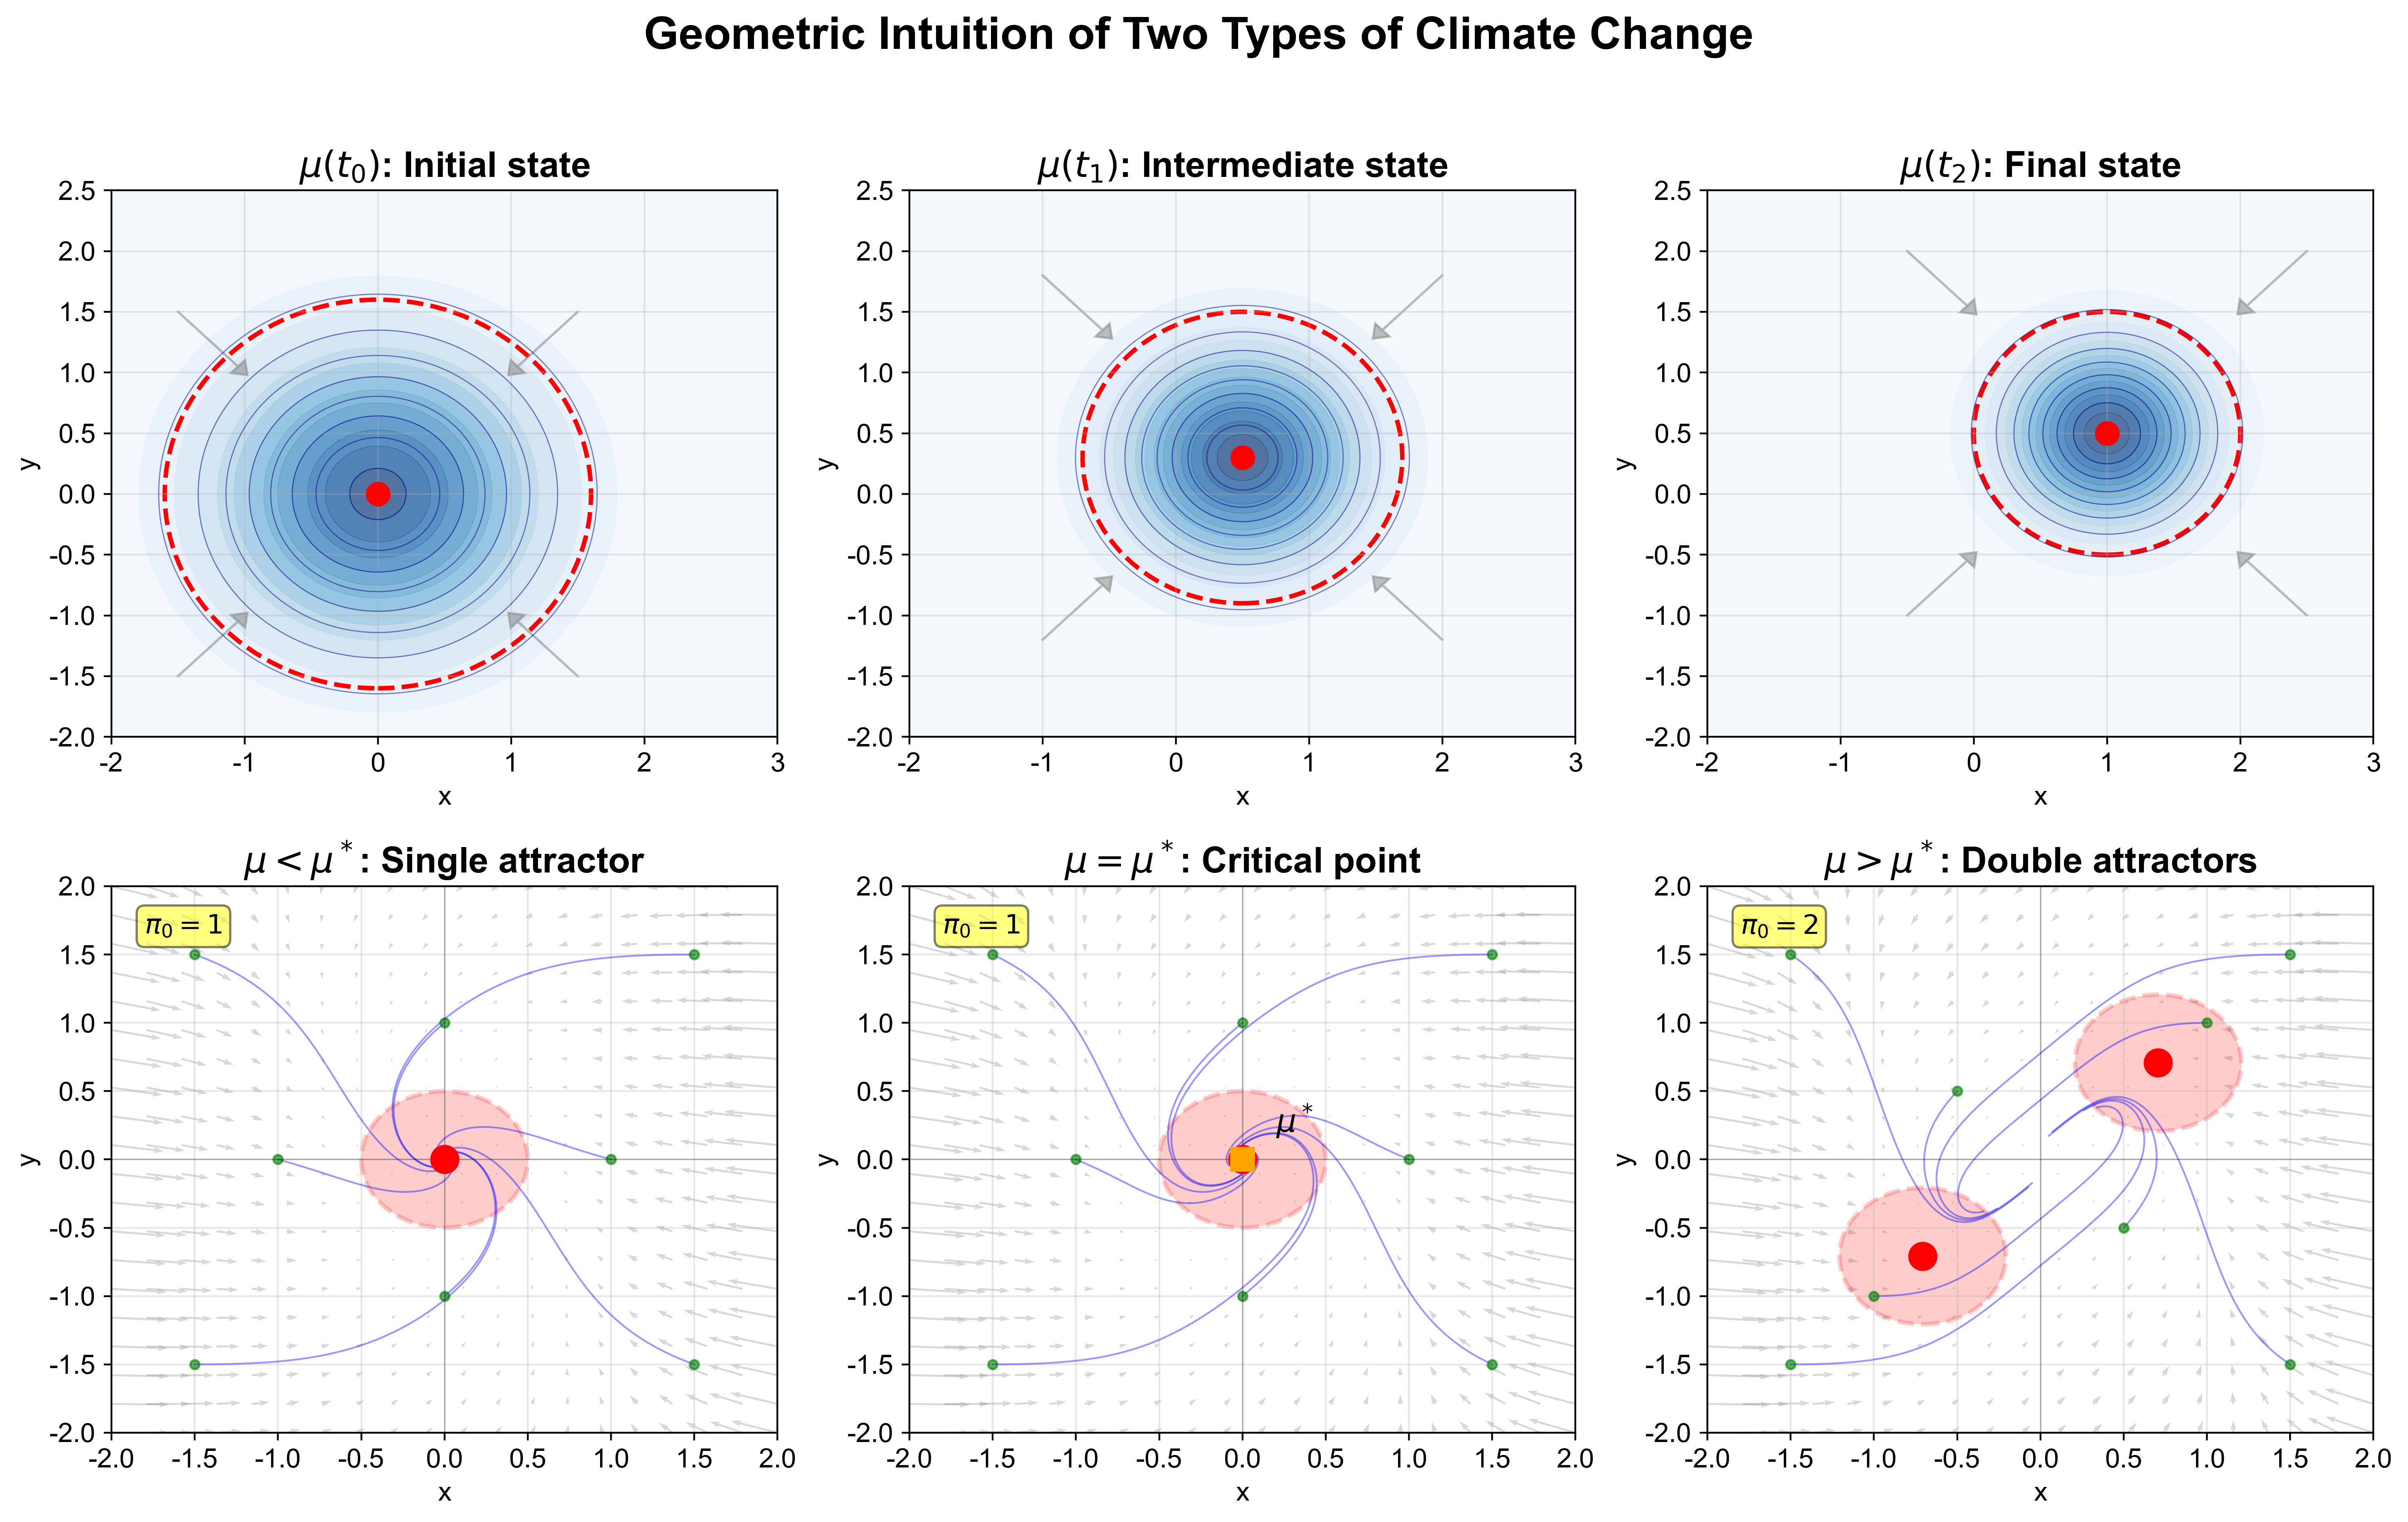
\includegraphics[width=0.9\textwidth]{./assets/climate_change_types.png}
    \caption{I类与II类气候变化的几何图景对比。上排: I类变化，吸引子 ($\pi_0 = 1$) 拓扑不变，概率测度在单个吸引子上重新分布，均值 $\mu$ 从 $\mu(t_0)$ 漂移到 $\mu(t_2)$。下排: II类变化，吸引子从单稳态 ($\pi_0 = 1$) 变为双稳态 ($\pi_0 = 2$)，产生了一个新的吸引子盆地，系统发生不可逆的跃迁。}
    \label{fig:climate_change_types}
\end{figure}

\subsection{I类气候变化: 概率测度的演化}

\begin{definition}[I类气候变化]
\label{def:type1_climate}
    若慢变量 $\slowvar(t)$ 在时间区间 $[t_0, t_1]$ 内演化，气候吸引子 $\attractor_{\slowvar(t)}$ 满足拓扑不变性:
    \begin{equation}
    \label{eq:type1_topology}
        H_*(\attractor_{\slowvar(t)}) \cong H_*(\attractor_{\slowvar(t_0)}), \quad \pi_0(\attractor_{\slowvar(t)}) = \text{const}, \quad \forall t \in [t_0, t_1]
    \end{equation}

    而流形度量 $\metric_{\slowvar(t)}$ 和概率测度 $\measure_{\slowvar(t)}$ 连续演化，则称系统发生I类气候变化。
\end{definition}

这里 $H_*$ 表示同调群 (Homology Groups)，$\pi_0$ 表示连通分量数 (Number of Connected Components)。
方程 \eqref{eq:type1_topology} 的数学意义是吸引子的个数和连通性保持不变。
原则上，I类变化具有可逆性: 若慢变量回复到初始值 $\slowvar(t_1) \to \slowvar(t_0)$，系统将回到初始气候状态。

\textbf{I类气候变化是当前气候系统的主要演化模式}。
其核心特征是概率测度 $\measure_{\slowvar}$ 随慢变量 $\slowvar$ 的演化。
我们首先说明，在I类变化中，吸引子拓扑保持不变，流形与度量的演化缓慢且效应不明显，但概率测度 $\measure_{\slowvar}$ 可以发生较显著的改变。

稳态Fokker-Planck方程 \eqref{eq:steady_fp} 的解 $\probdens_{ss}$ 由漂移向量场 $\drift$ 和扩散张量 $\difftensor$ 决定。
考虑一维系统 (可推广到高维情况)，不变概率测度满足 (参见 \cite{gardiner2009stochastic}):
\begin{equation}
\label{eq:steady_fp_solution}
    \probdens_{ss}(x; \slowvar) \propto \frac{1}{\difftensor(x; \slowvar)} \exp\left(\int^x \frac{2\drift(y; \slowvar)}{\difftensor(y; \slowvar)} dy\right)
\end{equation}

对 $\drift$ 求变分导数:
\begin{equation}
\label{eq:sensitivity_mean_partial_f}
    \frac{\delta \probdens_{ss}}{\delta \drift(z)} = \probdens_{ss}(x) \cdot \frac{2}{\difftensor(z)} \cdot H(x - z)
\end{equation}

其中 $H$ 是Heaviside函数。
因此:
\begin{equation}
    \frac{\partial \meanval}{\partial \drift(z)} = \int x \cdot \frac{\delta \probdens_{ss}}{\delta \drift(z)} dx = \frac{2}{\difftensor(z)} \int_{z}^{\infty} x \probdens_{ss}(x) dx \sim O(1/\difftensor)
\end{equation}

类似地，对 $\difftensor$ 求变分导数，可得:
\begin{equation}
    \frac{\partial \meanval}{\partial \difftensor(z)} \sim O(1/\difftensor^2), \quad \frac{\partial \sigma^2}{\partial \drift(z)} \sim O(1/\difftensor), \quad \frac{\partial \sigma^2}{\partial \difftensor(z)} \sim O(1/\difftensor^2)
\end{equation}

这表明，漂移向量场 $\drift$ 的微小改变 ($\Delta \drift$) 会导致均值和方差以 $O(1/\difftensor)$ 的速率变化；扩散系数 $\difftensor$ 的微小改变 ($\Delta \difftensor$) 会导致均值和方差以 $O(1/\difftensor^2)$ 的速率变化。
由于噪声强度 $\difftensor$ 相对较小，均值和方差对动力学参数的变化高度敏感。
微扰 ($\Delta \drift, \Delta \difftensor$) 将通过Fokker-Planck方程被“放大”为统计量的显著变化 ($\Delta \meanval, \Delta \sigma^2$)，这是\textbf{对气候变化非线性效应的动力学解释}。

概率测度 $\measure_{\slowvar}$ 的改变将对人类社会产生直接且重要的影响，尤其是尾部概率的变化，体现为\textbf{极端事件}频率的指数增长。

设 $\climind: \manifold \to \R$ 为气候指标 (温度、降水强度、风速等)，定义极端事件为 $\climind(\fastvar) > \threshold$，其中 $\threshold$ 为高阈值。
极端事件的发生概率由不变测度 $\probdens_{ss}$ 的尾部决定:
\begin{equation}
\label{eq:extreme_prob}
    P_{\text{extreme}}(\threshold; \slowvar) = \measure_{\slowvar}(\{\fastvar \in \manifold_{\slowvar} : \climind(\fastvar) > \threshold\}) = \int_{\climind(\fastvar) > \threshold} \probdens_{ss}(\fastvar; \slowvar) \, d\fastvar
\end{equation}

对应的\textbf{重现期 (Return Period)} 为:
\begin{equation}
\label{eq:return_period}
    T_{\text{return}}(\threshold; \slowvar) = \frac{1}{P_{\text{extreme}}(\threshold; \slowvar)}
\end{equation}

假设气候指标 $\climind(\fastvar)$ 近似服从正态分布:
\begin{equation}
\label{eq:normal_approx}
    \climind(\fastvar) \sim \mathcal{N}(\meanval(\slowvar), \sigma^2(\slowvar))
\end{equation}

其中 $\meanval(\slowvar) = \int \climind(\fastvar) \probdens_{ss}(\fastvar; \slowvar) d\fastvar$ 为均值；$\sigma^2(\slowvar) = \int (\climind(\fastvar) - \meanval)^2 \probdens_{ss}(\fastvar; \slowvar) d\fastvar$ 为方差。

对于高阈值 $\threshold \gg \meanval$，极端事件概率可用互补误差函数表示:
\begin{equation}
    \label{eq:extreme_prob_normal}
        P_{\text{extreme}}(\threshold; \slowvar) \approx \frac{1}{2}\mathrm{erfc}\left(\frac{\threshold - \meanval(\slowvar)}{\sqrt{2}\sqrt{\variance(\slowvar)}}\right) \sim \exp\left(-\frac{(\threshold - \meanval(\slowvar))^2}{2\variance(\slowvar)}\right)
    \end{equation}

慢变量变化 $\slowvar \to \slowvar'$ 导致概率测度的演化 $\measure_{\slowvar} \to \measure_{\slowvar'}$，从而改变均值 $\meanval$ 和方差 $\sigma^2$。
我们分别分析两种效应:

\textbf{(1) 均值漂移的影响}

若均值变化 $\meanval(\slowvar') = \meanval(\slowvar) + \Delta \meanval$ (不妨设 $\Delta \meanval > 0$)，方差不变，则尾部概率的相对变化为:
\begin{align*}
    \frac{P_{\text{extreme}}(\theta; \slowvar')}{P_{\text{extreme}}(\theta; \slowvar)} &= \exp\left(-\frac{(\theta - \meanval - \Delta\meanval)^2}{2\sigma^2} + \frac{(\theta - \meanval)^2}{2\sigma^2}\right) \\
    &= \exp\left(\frac{2(\theta - \meanval)\Delta\meanval - (\Delta\meanval)^2}{2\sigma^2}\right)
\end{align*}

当 $\Delta\meanval \ll \theta - \meanval$ 时，忽略二次项得:
\begin{equation}
\label{eq:extreme_prob_mean_shift}
    \frac{P_{\text{extreme}}(\threshold; \slowvar')}{P_{\text{extreme}}(\threshold; \slowvar)} \approx \exp\left(\frac{(\threshold - \meanval)\Delta \meanval}{\sigma^2}\right)
\end{equation}

由于 $\threshold \gg \meanval$，即使很小的均值变化 $\Delta \meanval$ 也会导致极端事件概率的显著增加。
取 $\theta - \meanval = 3\sigma$ (概率约千分之一)，若$\Delta\meanval = 0.1\sigma$，概率增加因子为 $\exp(3 \times 0.1) \approx 1.35$；若 $\Delta\meanval = \sigma$，增加因子将高达 $\exp(3) \approx 20$。

\textbf{(2) 方差增加的影响}

若方差变化 $\sigma^2(\slowvar') = \sigma^2(\slowvar) + \Delta \sigma^2$，均值不变，则尾部概率变化为:
\begin{equation*}
    \frac{P_{\text{extreme}}(\threshold; \slowvar')}{P_{\text{extreme}}(\threshold; \slowvar)} \approx \sqrt{\frac{\sigma^2}{\sigma^2 + \Delta\sigma^2}} \exp\left(\frac{(\threshold - \meanval)^2 \Delta \sigma^2}{2\sigma^2(\sigma^2 + \Delta\sigma^2)}\right)
\end{equation*}

当 $\Delta\sigma^2 \ll \sigma^2$ 时，主导项为:
\begin{equation}
\label{eq:extreme_prob_variance_increase}
    \frac{P_{\text{extreme}}(\threshold; \slowvar')}{P_{\text{extreme}}(\threshold; \slowvar)} \approx \exp\left(\frac{(\threshold - \meanval)^2 \Delta \sigma^2}{2(\sigma^2)^2}\right)
\end{equation}

方差增大将使概率测度尾部加厚 (Fat Tail)，分布更加扁平，极端值的概率密度更高。
由于 $\theta \gg \meanval$，即使方差的相对变化很小，极端事件概率也会显著增加。
若 $\theta - \meanval = 3\sigma$，方差增加 $10\%$ (即 $\Delta\sigma^2 / \sigma^2 = 0.1$)，概率增加因子约为 $\exp(9 \times 0.1 / 2) \approx 1.57$。

近年来，人类活动导致的气候变化已经导致了极端事件发生频率的极大提高。
以全球变暖为例，$\text{CO}_2$ 浓度从工业革命前的 $280$ ppm 升至当前的 $420$ ppm，全球温度均值升高约 $1.1$ °C，方差增加约 $15\%$ \cite{ipcc2021ar6}。
根据IPCC AR6报告 \cite{ipcc2021ar6}，$1.5$ °C的增温将使千年一遇的极端热浪变为百年一遇，重现期缩短10倍，对应概率增加10倍。
这正是均值漂移和方差增加带来的指数增长效应。

综上所述，我们从概率测度的角度定量分析了气候变化对极端事件概率的影响，揭示了动力学参数、概率测度和极端事件之间的关系链条:
\begin{equation*}
\Delta \drift, \Delta \difftensor \xrightarrow{\text{Fokker-Planck}} \Delta \meanval, \Delta \sigma^2 \xrightarrow{\text{尾部放大}} \Delta P_{\text{extreme}} \sim \exp(\cdot)
\end{equation*}

\subsection{II类气候变化: 拓扑突变与临界转变}

\begin{definition}[II类气候变化]
\label{def:type2_climate}
    若慢变量跨越临界值 $\slowvar^*$ 时，气候吸引子的拓扑结构发生间断改变:
    \begin{equation}
    \label{eq:type2_topology}
        H_*(\attractor_{\slowvar_-}) \not\cong H_*(\attractor_{\slowvar_+}), \quad \text{或} \quad \pi_0(\attractor_{\slowvar_-}) \neq \pi_0(\attractor_{\slowvar_+}), \quad \text{或} \quad \dim_H(\attractor_{\slowvar}) \text{跳跃}
    \end{equation}

    其中 $\slowvar_{\pm} = \slowvar^* \pm \epsilon$，则称系统发生II类气候变化，$\slowvar^*$ 为临界点 (Tipping Point)。
\end{definition}

II类变化对应动力系统的\textbf{分岔 (Bifurcation)}。
在临界点 $\slowvar^*$ 处，向量场 $\drift_{\slowvar}$ 的雅可比矩阵至少有一个特征值穿越虚轴 ($\mathrm{Re}(\eigenval) = 0$)，导致吸引子的稳定性发生质变。
常见的分岔类型包括:
\begin{enumerate}
    \item Saddle-node分岔: 其中吸引子与鞍点碰撞湮灭，系统跳跃到另一个吸引子 ($\pi_0: 2 \to 1$)；
    \item Hopf分岔: 稳定不动点失稳并产生极限环 (周期振荡)，拓扑维度增加 ($\dim_H: 0 \to 1$)；
    \item Pitchfork分岔: 单一吸引子分裂为两个对称吸引子，对称性自发破缺 ($\pi_0: 1 \to 2$)。
\end{enumerate}

\begin{figure}[htbp]
    \centering
    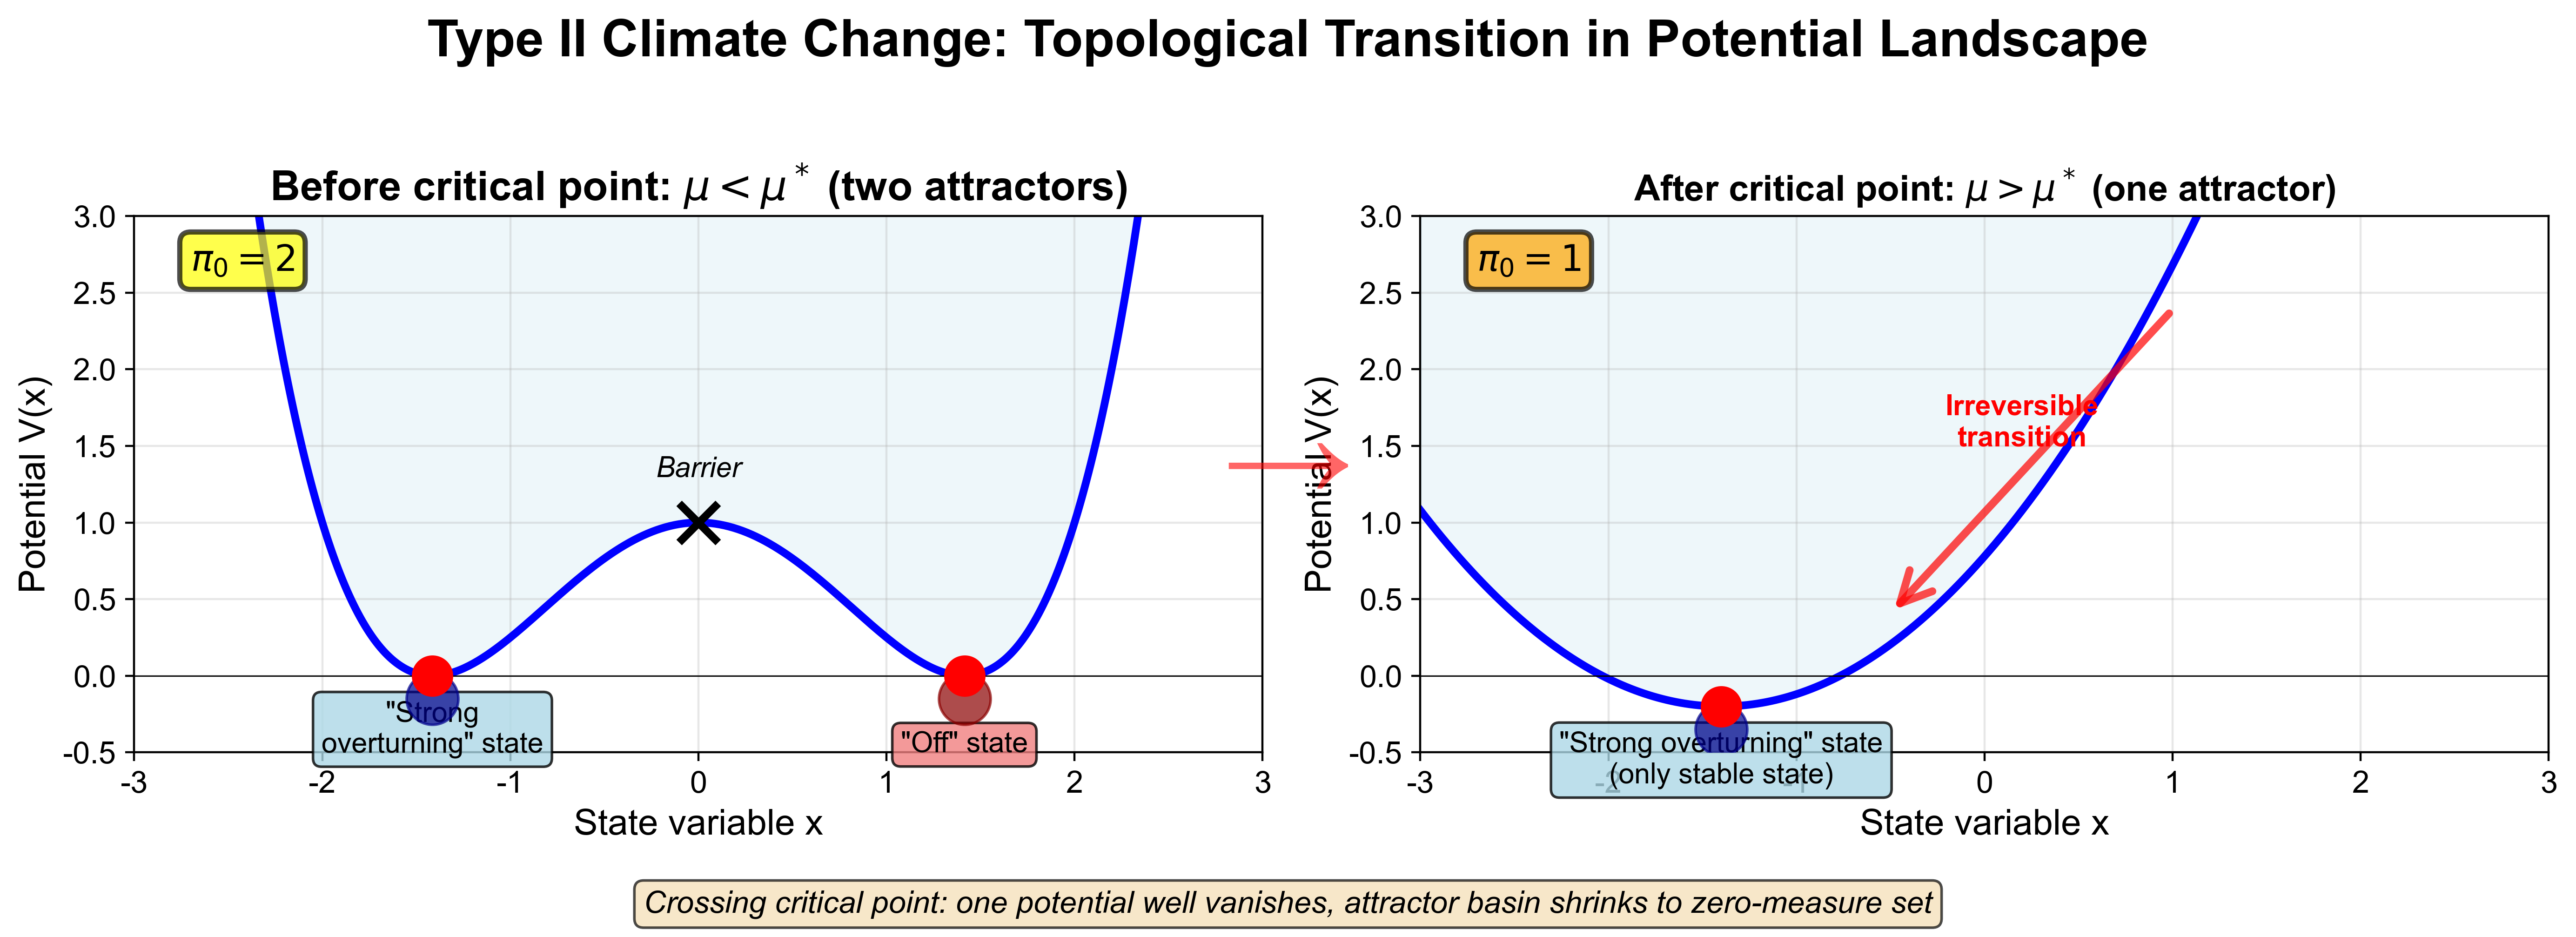
\includegraphics[width=1.00\textwidth]{./assets/potential_landscape_transition.png}
    \caption{Saddle-nod 分岔的势函数图景。左: 临界点前 ($\mu < \mu^*$)，双势阱对应两个吸引子 ($\pi_0 = 2$)态。右: 临界点后 ($\mu > \mu^*$)，右侧势阱消失，仅剩单一吸引子 ($\pi_0 = 1$)。}
    \label{fig:potential_landscape}
\end{figure}

II类变化的本质特征是不可逆性: 跨越临界点后，即使慢变量回复，系统也无法自动回到原来的吸引子，因为该吸引子已不复存在。

接近临界点时，系统将在多个层面呈现出可测量的\textbf{预警信号 (Early Warning Signals)} \cite{scheffer2009early}:
\begin{itemize}
    \item \textbf{临界慢化 (Critical Slowing Down)}:
    系统对扰动的恢复时间 $\predtime \sim 1/\sqrt{\eigenval} \to \infty$。
    具体表现为主导衰减模式的松弛率 $\eigenval_{\text{relax}} = -\mathrm{Re}(\eigenval_{\text{leading}}) \to 0^+$。
    \item \textbf{自相关增强 (Autocorrelation Enhancement)}:
    时间序列的滞后-1自相关系数趋近于1: $\mathrm{AC}(1) = \mathrm{Corr}(x_t, x_{t-1}) \to 1$，表明系统的“记忆”增强，状态转移减慢。
    临界点处 $\mathrm{AC}(1) \approx 1 - 2\eigenval_{\text{relax}}\Delta t$，可用于估计距临界点的距离。
    \item \textbf{方差发散}:
    概率测度向鞍点附近集中，导致状态变量的方差趋于无穷: $\mathrm{Var}[\fastvar] \to \infty$。
\end{itemize}

2009年，Rockström等学者提出了行星边界理论 (Planetary Boundaries theorem) \cite{rockstrom2009planetary}，认为地球系统存在9个临界子系统，即存在9个气候流形上的吸引子正在接近临界点 $\slowvar^*$。
这一理论为理解地球系统的稳态特性与气候变化的临界点提供了重要框架。

对于II类气候变化，我们介绍\textbf{大西洋经向翻转环流 (Atlantic Meridional Overturning Circulation, AMOC)} 的潜在崩溃作为典型案例。
AMOC是全球气候系统的关键组分，通过将热带暖水输送至北大西洋并驱动深层冷水南下，调节全球热量分布。
其驱动力来自北大西洋的密度差——表层海水在高纬度冷却增密并下沉，形成深层返流。然而，格陵兰冰盖融化释放的淡水正在降低海水盐度，从而减弱密度梯度并削弱环流强度。
当淡水通量超过临界阈值 $F^* \sim 0.1$ Sv时，系统将跨越临界点 \cite{stommel1961thermohaline,lenton2008tipping,dijkstra2005stability}。

从拓扑结构来看，AMOC存在两个吸引子态: “强翻转”态 ($\sim 20$ Sv，当前态) 和“弱翻转/关闭”态 ($< 5$ Sv)。
这对应两个独立的吸引子盆地 ($\pi_0 = 2$)。
临界点处，“强翻转”盆地在相空间中收缩至零测度集，随后消失 ($\pi_0: 2 \to 1$)，系统被迫不可逆跃迁至“关闭”态。
数学上，这是一个\textbf{Saddle-node分岔}，吸引子与鞍点在临界流形上碰撞湮灭。

观测数据为这一理论预测提供了有力支持。
Ditlevsen \& Ditlevsen (2023) \cite{ditlevsen2023warning} 分析了1870-2020年间的AMOC指标 (海温梯度、盐度剖面)，发现了多个临界预警信号。
自相关系数从1950年代的 $\mathrm{ACF}(1) \approx 0.7$ 增至2020年的 $\approx 0.9$，增幅达 $0.2$，这对应着松弛时间从 $20$ 年延长至 $100$ 年。
同时，方差增长率 $d\mathrm{Var}/dt > 0$ 且在1970年代后加速，符合临界慢化理论的预测。
基于这些信号，统计模型估计AMOC可能在2040-2070年间跨越临界点 ($95\%$置信区间)。

AMOC崩溃的全球影响将是灾难性的。
北欧地区将因失去暖流输送而温度下降 $3-5$ °C；热带辐合带将因大气环流重组而南移；美国东海岸将因海洋动力学高度变化而经历 $30-50$ cm的海平面上升；亚马逊和非洲萨赫勒地区将因远程气候耦合而降水减少 $20-40\%$。
这些变化对应着地球系统吸引子流形的拓扑重构，将影响数十亿人的生存环境 \cite{jackson2015global,ipcc2014ar5}。